\documentclass{article}
\usepackage{amsmath}
\usepackage{mathtools}
\usepackage{gensymb}
\usepackage[a4paper,inner=1.5cm,outer=1.5cm,top=2cm,bottom=0.5cm]{geometry} 
\usepackage{xcolor}                    
\usepackage{tikz}                           
\usepackage{multicol}
\usepackage{hyperref}
\usepackage{pgfplots}
\usetikzlibrary{calc}
\usetikzlibrary{intersections}
\usetikzlibrary{intersections,calc,angles,quotes}
\usetikzlibrary{shapes,arrows,positioning,decorations.pathreplacing,calc}
\usetikzlibrary{calc,angles,positioning,intersections,quotes,decorations.markings}
\usepackage{tkz-euclide}
\usetikzlibrary{backgrounds}
\usetikzlibrary{calc,through}
\usetikzlibrary{angles}
\usetikzlibrary{fadings}
\usetikzlibrary{shapes.geometric}
\usetikzlibrary{shapes.symbols}
\usepackage{draftwatermark}
\usepackage{mathptmx}

\SetWatermarkText{\textcolor{black!20}{Mathema Shukur}}
\SetWatermarkFontSize{2 cm}
\usepackage[utf8]{inputenc}
\usepackage{fontspec}

\setmainfont{[Kalpurush.ttf]}
\newfontface{\en}{[Arial.ttf]} %%this is optional, if you want to use a secondary font. Any english font is supported
\newlength\Radius
\setlength\Radius{4cm}
\begin{document} 
	\Large
	\textcolor{red}{Welcome To} 
	\\
	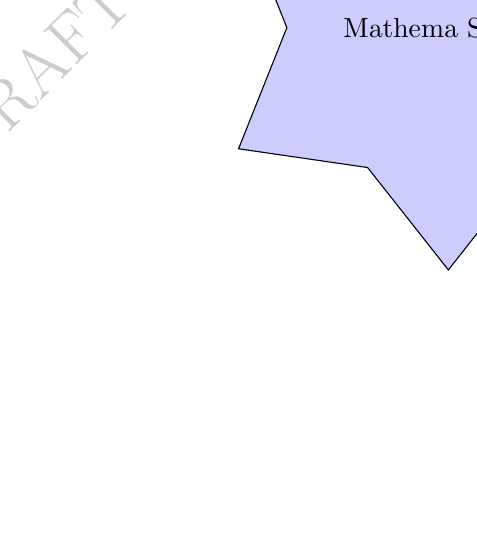
\begin{tikzpicture}
		\tikz \node [fill=blue!20,star,star points=6,draw] {Mathema Shukur };
	\end{tikzpicture}
	\\
	যাদের জন্যে প্রযোজ্যঃ  	\textcolor{magenta}{একাদশ ও দ্বাদশ শ্রেণীর শিক্ষার্থী} \\
	বিষয়ঃ \textcolor{magenta}{উচ্চতর গণিত ১ম পত্র} \\
	অধ্যায়ঃ \textcolor{magenta}{৪-বৃত্ত}\\ 
	\\
	\\
	\href{https://www.youtube.com/watch?v=DRxNte3mU6U&list=PLIjPH8h-K22w5iYZogyV1AI8-baSpY2Qn&index=1}{\textcolor{blue}{মূল বিন্দুতে (0,0) কেন্দ্র থাকলে বৃত্তের সমীকরণ কী?}}\\
	\\
\href{https://www.youtube.com/watch?v=rGCA1MltZsY&list=PLIjPH8h-K22w5iYZogyV1AI8-baSpY2Qn&index=2}{\textcolor{blue}{কী শর্তে কেন্দ্রের স্থানাঙ্ক হতে বৃত্তের ব্যাসার্ধ নির্ণয় করা হয়?}}\\
	\\
	\href{https://www.youtube.com/watch?v=gehIW-_0XrQ&list=PLIjPH8h-K22w5iYZogyV1AI8-baSpY2Qn&index=3}{\textcolor{blue}{বৃত্তের সাধারণ সমীকরণ $x^2+y^2+2gx+2fy+c=0$}}\\
	\\
		\href{https://www.youtube.com/watch?v=WzuG-MuA6Cs&list=PLIjPH8h-K22w5iYZogyV1AI8-baSpY2Qn&index=4}{\textcolor{blue}{পোলার স্থানাঙ্কে বৃত্তের সমীকরণ নির্ণয়}}\\
		\\
			\href{https://www.youtube.com/watch?v=ssCuBx7HEHI&list=PLIjPH8h-K22w5iYZogyV1AI8-baSpY2Qn&index=5}{\textcolor{blue}{ব্যাসের প্রান্ত বিন্দু (x1,y1) ও (x2,y2) হলে বৃত্তের সমীকরণ নির্ণয়}}\\
			\\
				\href{https://www.youtube.com/watch?v=afVjGQrIpDs&list=PLIjPH8h-K22w5iYZogyV1AI8-baSpY2Qn&index=6}{\textcolor{blue}{বৃত্ত ও সরলরেখার ছেদবিন্দুগামী বৃত্তের সমীকরণ}}\\
			\\
				\href{https://www.youtube.com/watch?v=rXOyjYE6YfU&list=PLIjPH8h-K22w5iYZogyV1AI8-baSpY2Qn&index=7}{\textcolor{blue}{দুইটি বৃত্তকে ছেদ করে এমন বৃত্তের সমীকরণ}}\\
		\\
	\textcolor{magenta}{৩ টি বিন্দুগামী বৃত্তের সমীকরণ নির্ণয় }\\
	\\
	একটি বৃত্তের সমীকরণ নির্ণয় কর যা \textcolor{blue}{$(1,-6)$,$(2,1)$} এবং \textcolor{blue}{$(5,2)$}  বিন্দুগামী। \\ 
	\\
	\begin{tikzpicture}[transform shape,scale=1]
		\draw [-latex,thick,red](-1,0) -- (11,0) node[right] {$x$} coordinate(x axis);
		\draw [-latex,thick,red](0,-9) -- (0,3) node[above] {$y$} coordinate(y axis);
		\fill[black] (0,0) circle (1 mm);
		\node at (0.8,-0.3) {$\textcolor{red}{O(0,0)}$};	
		\draw[thick,green] (5,-3) circle (5);
		\fill[blue] (1,-6) circle (1 mm);
		\node at (1,-6.5) {$\textcolor{blue}{(1,-6)}$};
		\fill[blue] (2,1) circle (1 mm);
		\node at (2,1.5) {$\textcolor{blue}{(2,1)}$};
		\fill[blue] (5,2) circle (1 mm);
		\node at (5,2.5) {$\textcolor{blue}{(5,2)}$};
	\end{tikzpicture}\\
	\\
	বৃত্তের সাধারণ সমীকরণ \\ 
		\begin{align*}
		x^2+y^2+2gx+2fy+c&=0
	\end{align*}
\\
	বৃত্তের সাধারণ সমীকরণে $(1,-6)$ বিন্দুটি বসিয়ে পাই  \\ 
	\begin{align*}
			x^2+y^2+2gx+2fy+c&=0\\
			\boxed{\textcolor{blue}{x=1,\,\,y=-6}}&\\
	(1)^2+(-6)^2+2g(1)+2f(-6)+c&=0\\
	\\
	1+36+2g-12f+c&=0\\
	\\
	2g-12f+c&=-37\,\,\,[EQ01]\\
\end{align*}
\\
	বৃত্তের সাধারণ সমীকরণে $(2,1)$ বিন্দুটি বসিয়ে পাই  \\ 
\begin{align*}
		x^2+y^2+2gx+2fy+c&=0\\
		\boxed{\textcolor{blue}{x=2,\,\,y=1}}&\\
	(2)^2+(1)^2+2g(2)+2f(1)+c&=0\\
	\\
	4+1+4g+2f+c&=0\\
	\\
	4g+2f+c&=-5\,\,\,[EQ02]\\
\end{align*}
\\
	বৃত্তের সাধারণ সমীকরণে $(5,2)$ বিন্দুটি বসিয়ে পাই  \\ 
\begin{align*}
		x^2+y^2+2gx+2fy+c&=0\\
		\boxed{\textcolor{blue}{x=5,\,\,y=2}}&\\
	(5)^2+(2)^2+2g(5)+2f(2)+c&=0\\
	\\
25+4+10g+4f+c&=0\\
	\\
10g+4f+c&=-29\,\,\,[EQ03]\\
\end{align*}
\\
\begin{align*}
	2g-12f+c&=-37\,\,\,[EQ01]\\
	\\
		4g+2f+c&=-5\,\,\,[EQ02]\\
		\\
		10g+4f+c&=-29\,\,\,[EQ03]\\
\end{align*}
\\
১ নং সমীকরণ হতে ২ নং সমীকরণ বিয়োগ করে পাই\\ 
\begin{align*}
	(2g-12f+c)-(4g+2f+c)&=-37-(-5)\,\,\,\,[EQ01-EQ02]\\
	\\
2g-12f+c-4g-2f-c&=-32\\ 
	\\
-2g-14f&=-32\\
\\
g+7f&=16\,\,\,[EQ04]
\end{align*}
\\
২ নং সমীকরণ হতে ৩ নং সমীকরণ বিয়োগ করে পাই\\ 
\begin{align*}
(4g+2f+c)-(	10g+4f+c)&=-5-(-29)\,\,\,[EQ02-EQ03]\\
	\\
	4g+2f+c-10g-4f-c&=24\\
	\\
-6g-2f&=24\\
\\
3g+f&=-12\,\,\,[EQ05]
\end{align*}
\\
৪ নং সমীকরণের সাথে ৫ নং সমীকরণ যোগ করে পাই \\ 
\begin{align*}
(g+7f)+(3g+f)&=16+(-12)\,\,\,[EQ04]+[EQ05]\\
	\\
4g+8f&=4\\
	\\
g+2f&=1\\ 
\\
g=&1-2f\,\,\,[EQ06]
\end{align*}
\\
\begin{align*}
g+7f&=16\,\,\,[EQ04]\\
\\
1-2f+7f&=16\\
\\
5f&=15\\
\\
f&=3
\end{align*}
\\
\begin{align*}
g=&1-2f\,\,\,[EQ06]\\
	\boxed{\textcolor{blue}{f=3}}&\\
g=&1-2(3)\\
\\
g=&-5
\end{align*}
\\
\begin{align*}
	2g-12f+c&=-37\,\,\,[EQ01]\\
	\boxed{\textcolor{blue}{g=-5,\,\,f=3}}&\\
2(-5)-12(3)+c&=-37\\
\\
-10-36+c&=-37\\
\\
c&=9
\end{align*}
\\
বৃত্তের সাধারণ সমীকরণে $g,\,\,\,f,\,\,\,c$  এর মান বসিয়ে পাই \\ 
\begin{align*}
	x^2+y^2+2gx+2fy+c&=0\\
	\\
		\boxed{\textcolor{blue}{g=-5,\,\,f=3,\,\,\,c=9}}&\\
		\\
		x^2+y^2+2(-5)x+2(3)y+9&=0\\
		\\
	\textcolor{green}{x^2+y^2-10x+6y+9=0}&	\\	
\end{align*}
\\
\textcolor{red}{[চট্রগ্রাম বোর্ড-২০১৮]}\\ 
	একটি বৃত্তের সমীকরণ নির্ণয় কর যা \textcolor{blue}{$(4,2)$,$(-1,4)$} এবং \textcolor{blue}{$(-3,4)$}  বিন্দুগামী \\ 
	\\
	\textcolor{red}{[দিনাজপুর বোর্ড-২০১৭]}\\ 
	একটি বৃত্তের সমীকরণ নির্ণয় কর যা \textcolor{blue}{$(-6,5)$,$(-3,-4)$} এবং \textcolor{blue}{$(2,1)$}  বিন্দুগামী \\ 
	\\
	\textcolor{red}{[বরিশাল বোর্ড-২০১৭]}\\
	একটি বৃত্তের কেন্দ্র $\textcolor{blue}{x+2y+1=0}$ রেখার উপর অবস্থিত এবং যা মূলবিন্দু ও $\textcolor{blue}{x^2+y^2+3x-5y+6=0}$ বৃত্তের কেন্দ্র দিয়ে যায় । বৃত্তটির সমীকরণ নির্ণয় কর।  \\
	\\ 
		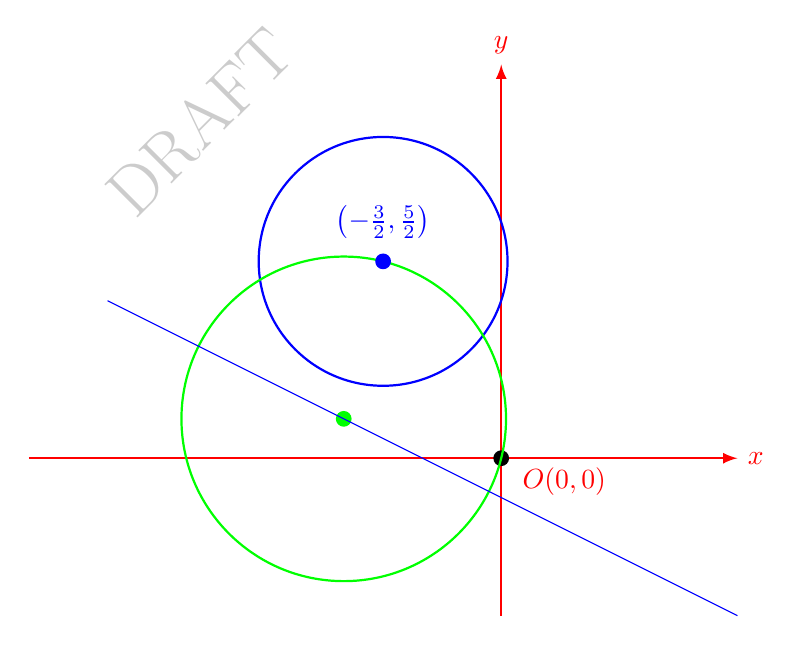
\begin{tikzpicture}[transform shape,scale=1]
		\draw [-latex,thick,red](-6,0) -- (3,0) node[right] {$x$} coordinate(x axis);
		\draw [-latex,thick,red](0,-2) -- (0,5) node[above] {$y$} coordinate(y axis);
		\fill[black] (0,0) circle (1 mm);
		\node at (0.8,-0.3) {$\textcolor{red}{O(0,0)}$};
		\draw[thick,blue] (-1.5,2.5) circle (1.58);	
		\draw[thick,green] (-2,0.5) circle (2.061);
			\fill[green](-2,0.5) circle (1 mm);
		\fill[blue] (-1.5,2.5) circle (1 mm);
		\node at (-1.5,3) {$\textcolor{blue}{\left(-\frac{3}{2},\frac{5}{2}\right)}$};
		\draw[blue](-5,2)--(3,-2);
	\end{tikzpicture}\\
	\\
মূলবিন্দুগামী বৃত্তের $(c=0)$ সমীকরণ \\
	\begin{align*}
		x^2+y^2+2gx+2fy+0&=0\\
		\\
			x^2+y^2+2gx+2fy&=0\,\,\,[EQ01]\\
	\end{align*}
\\
যেহেতু ১নং বৃত্তটি  $x^2+y^2+2\left(\frac{3}{2}\right)x+2\left(-\frac{5}{2}\right)y+6=0$ বৃত্তের কেন্দ্র $\left(-\frac{3}{2},\frac{5}{2}\right)$ দিয়ে যায় \\
\\
\begin{align*}
	x^2+y^2+2gx+2fy&=0\\
	\boxed{\textcolor{blue}{x=\left(-\frac{3}{2}\right),\,\,\,y=\left(\frac{5}{2}\right)}}&\\
	\left(-\frac{3}{2}\right)^2+\left(\frac{5}{2}\right)^2+2g\left(-\frac{3}{2}\right)+2f\left(\frac{5}{2}\right)&=0\\
	\\
	\left(\frac{9}{4}\right)+\left(\frac{25}{4}\right)-3g+5f&=0\\
	\\
9+25-12g+20f&=0\\
\\
-12g+20f&=-34\\
\\
6g-10f&=17\,\,\,[EQ02]
\end{align*}
\\
১ নং বৃত্তের কেন্দ্র $(-g,-f)$, $x+2y+1=0$ রেখার উপর অবস্থিত \\
\\
\begin{align*}
	x+2y+1&=0\\
	\\
		\boxed{\textcolor{blue}{x=-g,\,\,y=-f}}&\\
		\\
		(-g)+2(-f)+1&=0\\
		\\
		g+2f&=1\\
		\\
		g&=1-2f\,\,\,\,[EQ03]
\end{align*}
\\
\begin{align*}
6g-10f&=17\,\,\,[EQ02]\\
\\
6(1-2f)-10f&=17\\
\\
6-12f-10f&=17\\
\\
-22f&=11\\
\\
f&=-\frac{1}{2}
\end{align*}
\\
\begin{align*}
	g&=1-2f\,\,\,\,[EQ03]
	\\
		g&=1-2\left(-\frac{1}{2}\right)\\
		\\
		g&=1+1\\
		\\
		g&=2
\end{align*}
১ নং বৃত্তের সমীকরণে $g,\,\,\,f$ এর মান বসিয়ে পাই 
\\
\begin{align*}
	x^2+y^2+2gx+2fy&=0\\
	\\
		x^2+y^2+2(2)x+2\left(-\frac{1}{2}\right)y&=0\\
		\\
	\textcolor{green}{x^2+y^2+4x-y=0}&	
\end{align*}
\end{document}